% Finnish or English, gives the right language to title page and Finnish enables special chars ä ö å.
\documentclass[a4paper,finnish,12pt]{article}
\bibliographystyle{ieeetr}
\usepackage[T1]{fontenc}
\usepackage[utf8]{inputenc}
\usepackage[finnish]{babel}

\usepackage{mathtools}
%\usepackage[lstlisting]{/home/micsu/Dropbox/Opinnot/gittisetit/LaTeX/mcode}
\usepackage{amsfonts,amssymb,amsbsy}
\usepackage{fancyhdr}
\usepackage[a4paper]{geometry}
%\usepackage[RGB,ELEC]{/home/micsu/Dropbox/Opinnot/gittisetit/LaTeX/aaltologo}
\usepackage{graphicx}
\usepackage{caption}
\usepackage{subcaption}

\begin{document}

\thispagestyle{empty}

\begin{titlepage}
    \centering
    \vspace*{10\baselineskip}
    \Large
    \bfseries
    AS-0.3100 \\ Automaatio ja systeemitekniikan seminaari \\
    \vspace{\baselineskip}
    \huge
    Osaamisen kehittymisen hallinta \\
    [1.5\baselineskip]
    \normalfont
    \vfill
    \small
    Automaatio- ja systeemitekniikka \\
    \vfill
    Miikka Eloranta \\
    80294A \\[2\baselineskip]
    \textbf{\today} \\[2\baselineskip]
    \vfill
%	\AaltoLogoSmall{1}{?}{aaltoPurple}


\end{titlepage}

% DOCUMENT START

\pagebreak

\tableofcontents

\pagebreak

\section{Johdanto}

Motivaatio lyhyesti.

Keskitytään ICT-palveluyrityksiin.

Toisessa luvussa esitellään tarkemmin motivaatio osaamisten keskitettyyn jatkuvan kehittymisen hallintaan. Kolmannessa luvussa käsitellään tarkemmin osaamisen määritystä, sen mittausperusteita ja jaottelua. Sen lisäksi kolmannessa luvussa esitellään visuaalisesti hyvin havainnollistava T-malli henkilön työroolikohtaisten osaamisten esitykseen. Neljäs luku käsittelee osaamisten kehittymistä, erilaisia kehityksen perusteita ja sen suunnittelua. Viides luku tarjoaa lyhyen katsauksen osaamisten kehittymisen seurantaan ja hallintaan tarkoitetun työkalun tarjoamista mahdollisuuksista.

\pagebreak

\section{Motivaatio}

Yritysmaailmassa oman työnsä tehostamiseksi on muiden työntekijöiden lisäksi hyvä tuntea myös kollegoiden osaamisalueet. Pienikokoisissa yrityksissä, pienissä startupeissa tai yksittäisenä yrittäjänä toimiessa tämä on helppoa, koska ihmisiä on vähän tai yksittäisenä yrittäjänä oman osaamisalueen ulkopuoleiseen tekemiseen valitaan juuri siihen aihealueeseen erikoistunut kumppani. Pienyrityksessä kullakin on tarkka vastuualue ja jokainen on osaltaan tärkeä kokonaisuuden kannalta, joten osaamisalueiden tuntemus on oman työnkin kannalta ehdoton vaatimus. Suurissa ja etenkin nopeasti henkilöstömäärällisesti kasvavissa yrityksissä muiden työntekijöiden -- saati näiden kunkin osaamisalueen -- tuntemus on sen sijaan selvästi hankalampaa.

Kollegoiden osaamisten tuntemisen tärkeys korostuu ennen kaikkea asiantuntijuuteen keskittyneisiin palveluyrityksiin. Kovassa kilpailutuksessa on osattava kertoa laajemmin koko yrityksen osaamistarjonnasta ja myös olemassa olevien asiakkaiden muuttuviin tarpeisiin on pystyttävä reagoimaan nopeasti -- joko etsimällä tarpeen täyttävä osaaja yrityksen sisältä, rekrytoimalla tai kehittämällä osaamista. Koska kuitenkaan kaikkien yksittäisten asiakkaiden tarpeiden muuttuessa ei osaamista voi välttämättä kehittää tarpeiden mukaan, on osaamisen kehittämistä osattava ennakoida ja valita tärkeimmän kehityssuunnat.

Sen lisäksi, että kollegoiden osaaminen on hyvä tuntea, tulee koko yrityksen osaamistarjonnan olla keskitetysti hallittua, jotta lukumäärällisesti voidaan nopeasti ilmoittaa tietyn osaamisen hallitsevat henkilöt. Monesti asiakkaan kilpailuttaessa palveluyrityksiä tullaan varmistamaan, että tällä on riittävästi asiakkaan tarpeet täyttäviä osaajia.

Teknologiaosaamisten osalta korkean luokan asiantuntijuus ei saisi keskittyä laajalta osin liian pieneen osaan yrityksen henkilöstöä. Vaikka eri työrooleissa asiantuntijuuden syvyys vaihtelee laajalti, ei yksittäinen henkilö saa olla omassa roolissaan korvaamaton. Siinä missä asiakaspalvelija voi vastata laajalti eri teknologioihin tai asiakasympäristöihin liittyvistä perusongelmista, täytyy jollain olla osaamista myös tarkasti kunkin ympäristön arkkitehtuurista. Kuitenkin, jos yksi ja sama henkilö on suunnitellut ja rakentanut kaikkien asiakasympäristöjen tietyt osa-alueet, kostautuu tämä valtavana ongelmana esim. henkilön irtisanoutuessa.

Osaamiset on siis saatava hallitusti jaettua laajemmalle määrälle henkilöstöä pitäen kuitenkin mielessä kunkin työroolin kannalta olennaiset osaamistasot ja alueet. Jotta näitä saadaan hallitusti ja jatkuvasti seurattua ja kehitettyä, on kaikkea henkilöstön osaamista hallittava keskitetysti. Koska kaiken olemassaolevan osaamisen lisäksi sitä on myös kehitettävä, tulee myös kehittämisen olla suunnitelmallista ja suunnitelmia ylläpidettävä tässä yhteydessä yhtä lailla.

\pagebreak

\section{Osaaminen -- mitä käytännössä?}

Siinä, missä osaamista voi kasvattaa itse tekemällä tai koulutuksia käymällä, palveluyritysmaailmassa selkeimmät ``merkinnät'' omasta osaamisesta ovat suoritetut sertifioitumiset ja referenssit, jossa asiakkaalta voi varmistaa, että kyseinen henkilö on toiminut tietyssä projektissa tietyssä tehtävässä toteuttaen tiettyjä toimia, tietyillä teknologioilla jne. Sertifioitumiset koostuvat yhdestä tai useammasta suoritetusta testistä, jotka suoritetaan yleensä varsinaisen koulutuksen jälkeen. Käytännössä siis henkilö osoittaa, että on oppinut koulutuksen aihealueen ja ``validoituu'' kyseisen aihealueen osaajaksi.

Varsinainen käytännön osaaminen ei kuitenkaan kartu pelkillä teoriaopinnoilla. Vaikka koulutuksessa todennäköisimmin onkin myös käytännön tekemistä, voi sertifikaattitestejä suorittaa myös ilman varsinaiseen koulutukseen osallistumista. Lisäksi voi olla osaajia, jotka eivät ole vielä sertifioituneet tietyn osaamisen osaajiksi -- joko tähän ei ole ollut aikaa tai henkilö ei yksinkertaisesti menesty teoreettisistä testeissä samalla tasolla kuin käytännön osaamisen saralla -- ja toisaalta on osaamisia, joihin ei yksinkertaisesti voi sertifioitua. Osaaminen pitäisi siis määritellä yleisemmällä tasolla. 

Palveluyrityksen valinnassa sertifikaattien ja työkokemuksen lisäksi asiakasyrityksen tulee huomioida sen kumppanit, kumppanuustasot ja olemassa olevat asiakkaat  -- ennen kaikkea lukeutuuko nykyasiakkaisiin saman toimialan yrityksiä \cite{ICT-haasteet}.

\subsection{Jaottelu}

Madhavan et. Al tunnisti osaamisisten mittaroinnissa useamman ulottuvuuden. Niin kutsutussa T-mallissa leveys kuvaa osaamisten kokonaismäärää ja korkeus niiden syvyyttä. Mikäli asiantuntijan osaaminen keskittyy esimerkiksi tiettyyn teknologiaan, on hänen osaamisten T-mallissaan kapea, mutta korkea piikki. T-mallia käytetään osaamisten jaottelemiseksi tiettyihin kokonaisuuksiin. \cite{ICT-haasteet}

Tässä ICT-palveluyrityksille tarkoitetussa T-mallissa osaamiset on jaoteltu seuraavasti: \begin{enumerate}
	\item Henkilökohtaiset kyvykkyydet
	%\begin{itemize}
		%\item Kielitaidot
		%\item Tiimityöskentelytaidot
		%\item Paineensietokyky
		%\item \ldots
	%\end{itemize}
	\item Organisaatio- ja toimialakohtaiset osaamiset
	%\begin{itemize}
		%\item Yrityksen kumppanit ja kumppanuustasot
		%\item Kilpailijat
		%\item Asiakkaan edustajien tuntemus
		%\item \ldots
	%\end{itemize}
	\item Ammatilliset ja teknologiaosaamiset.
	%\begin{itemize}
		%\item Microsoft Exchange 2008
		%\item J2EE-ohjelmointi
		%\item Asiakkaan X järjestelmän Y arkkitehtuuri
		%\item \ldots
	%\end{itemize}
\end{enumerate} Kuvassa \ref{fig:Tareas} on esitetty edellä listattujen osaamisalueiden sijainnit T-mallilla. Henkilökohtaisiin kyvykkyyksiin määritellään kaikki henkilön omaan käyttäytymiseen, muiden kanssa kommunikointiin ja kyvykkyyteen toimia tietyissä rooleissa. Näihin kuuluvat muun muassa kielitaidot, tiimityöskentelytaidot tai paineensietokyky. Organisaatio- ja toimialakohtaisiin osaamisiin taas määritelään mm. kaikki yrityksen käytäntöihin liittyvät osaamiset, kilpailijat, kumppanit ja kumppanuustasot, sekä asiakkaan edustajien tuntemus. Viimeisenä ammatillisiin ja teknologiaosaamisiin liittyy kaikki eri teknologioihin, ohjelmointikieliin ja -kehitykseen, asiakkaiden järjestelmien arkkitehtuureihin yms. liittyvät osaamiset. T-malli on valittu, koska osa-alueita on kolme ja kukin sen osio kuvaa yhtä osa-alueista.

\begin{figure}[t]
	\centering
	\begin{subfigure}[t]{0.45\textwidth}
		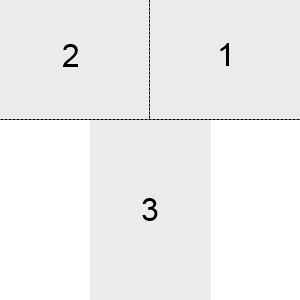
\includegraphics[width=\textwidth]{T_areas.png}
		\caption{Käytetyt osaamisaluejaot ICT-palveluyritykselle.}
		\label{fig:Tareas}
	\end{subfigure}
	\hfill
	\begin{subfigure}[t]{0.45\textwidth}
		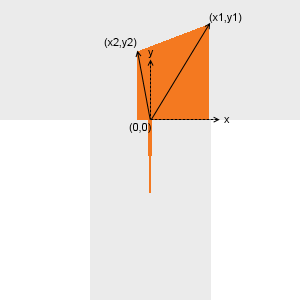
\includegraphics[width=\textwidth]{T_drawing_logics.png}
		\caption{Piirtologiikka valitulle työroolille.}
		\label{fig:Tlogics}
	\end{subfigure}
	\caption{T-mallin osaamisalueet ja piirtologiikka.}
\end{figure}

Koska kullakin työroolilla kaivataan erityyppisiä osaajia, T-mallia piirrettäessä sen kukin haara skaalataan rooliin vaadittavien osaamisten mukaisesti. T-mallin yläosa piirretään käyttäen yhtälöparin %\eqref{Tlogics_optim} ja \eqref{Tlogics} mukaisella logiikalla, joka on myös esitetty kuvassa \ref{fig:Tlogics}. Taustalla näkyvä harmaa T on valitun työroolin ``optimi-T,'' joka pitää sisällään kaikki työroolin osaamiset. Harmaa T-malli skaalataan osaamisten lukumäärien mukaisesti symmetriseksi yhtälön \eqref{Tscaleconstants} mukaisesti ja näin saatuja skaalauskertoimia käytetään henkilön T-mallin piirrossa. Yhtälön \eqref{Tscaleconstants} muuttuja $A_1$ on skaalauskerroin henkilökohtaisten kyvykkyyksien leveydelle, $A_2$ vastaavasti organisaatio- ja toimialakohtaisten osaamisten leveyksille ja $B_1$ sekä $B_2$ vastaavat korkeusskaalaimet.
\begin{equation}
\begin{cases}
A_i = 1/n_i \\
B_i = 1/5 \\
\end{cases}
\label{Tscaleconstants}
\end{equation} skaalauskertoimia, jossa $A_i$ on osaamisalueen $i$ skaalauskerroin leveydelle ja $n_i$ vastaavan alueen osaamisten kokonaislukumäärä. $B_i$ on vastaavasti korkeuden skaalauskerroin, joka on kaikille $1/5$, koska osaamistasoja on tässä määritelty viisi kappaletta ja korkeus määritetään henkilölle määriteltyjen osaamisten tasojen keskiarvona.

Käyttäen kertoimia yhtälöstä \eqref{Tscaleconstants} saadaan henkilölle määriteltyä kuvan \ref{fig:Tlogics} mukaiset pisteet $(x_1, y_1)$ ja $(x_2, y_2)$ yhtälöllä
\begin{equation}
\begin{cases}
x_i = (-1)^{i-1} \cdot O_i / n_i \\
y_i = \bar{O_i} = \sum_{k \in O_i} \frac{O_i}{n_i}, \\
\end{cases}
\end{equation} jossa $O_i$ kattaa henkilölle määritetyt osaamiset osaamisalueessa $i$.


T-malli höpöhöpö \cite{T-malli}.

Miten jaotellaan / miksi pitää jaotella?

T-malli, hyvää/huonoa

Teknologiaosaamisten laajuus, kuinka tarkentaa?

Teknologia itsessään / asiakasympäristön syväosaaminen

\pagebreak

\section{Jatkuva kehittyminen}

Osaamisen kehittyminen on jatkuva prosessi. Kun teknologiat, prosessit ja menetelmät kehittyvät, asiakkaat haluavat siirtyä niihin. Tämän tarpeen seurauksena palveluyrityksen asiantuntijat kouluttautuvat niihin, osaaminen näihin kasvaa ja tarpeet saadaan täytettyä. Koska kuitenkin tämän seurauksena teknologian osaajien määrä ja tietoisuus siitä maailmalla kasvaa, myös teknologian kehittäjä saa lisää mahdollisuuksia jatkokehittää sitä. Melko ylätason kuvaus tästä jatkuvasta prosessista on esitetty kuvassa \ref{fig:perusympyra}. Luonnollisesti myös palveluyrityksessä henkilöstö muuttuu ja näistä aiheutuu mahdollisisti kehitystarpeita tai niiden täyttymisiä. Ne on esitetty kuvassa katkoviivalla. Vaikka tarpeita uusien teknologioiden osaamiseen ei suoraan olemassaolevilta asiakkailta tulisikaan, palveluyritysten kilpailun vuoksi yriyksen on pidettävä oma osaamisensa jatkuvasti ajan tasalla säilyttääkseen kilpailukykynsä.

\begin{figure}[ht]
\centering
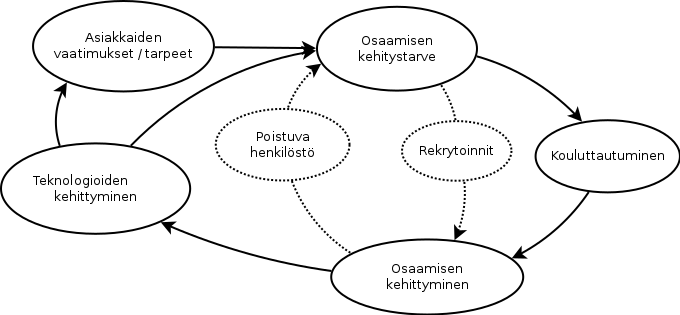
\includegraphics[scale=0.5]{knowledge_circle.png}
\caption{Osaamisen jatkuva kehittäminen}
\label{fig:perusympyra}
\end{figure}

Uudet teknologiat, kasvava yritys, vitusti pilvee Kalliosta

\subsection{Kehittymisen suunnittelu}

Koko organisaation kehityssuunnat määrittyvät yksilöiden kautta. Vaikka organisaatiolla olisikin tietyt tavoitteet kehityssuunniksi, sen toteutuminen on riippuvaista siitä, onko osaamisen kehitystä hankkiva henkilökunta motivoitunutta. Tästä syystä henkilöstön itsensä tulee saada olla vaikuttamassa oman henkilökohtaisen koulutus- ja kehityssuunnitelmansa tekoon.

\pagebreak

\section{Mikä vitun Akatemia?}

"Akatemia" yleisenä terminä vai tuotehöpinää?

\pagebreak

\section{Yhteenveto ja johtopäätökset}

Vittuun työt ja vittuun työkkäri

\pagebreak


\clearpage

%% Lähdeluettelo
\addcontentsline{toc}{section}{Viitteet}
\bibliography{refet}

\appendix


\end{document}
